\section{Motoren}
\begin{figure}[h]
    \centering
    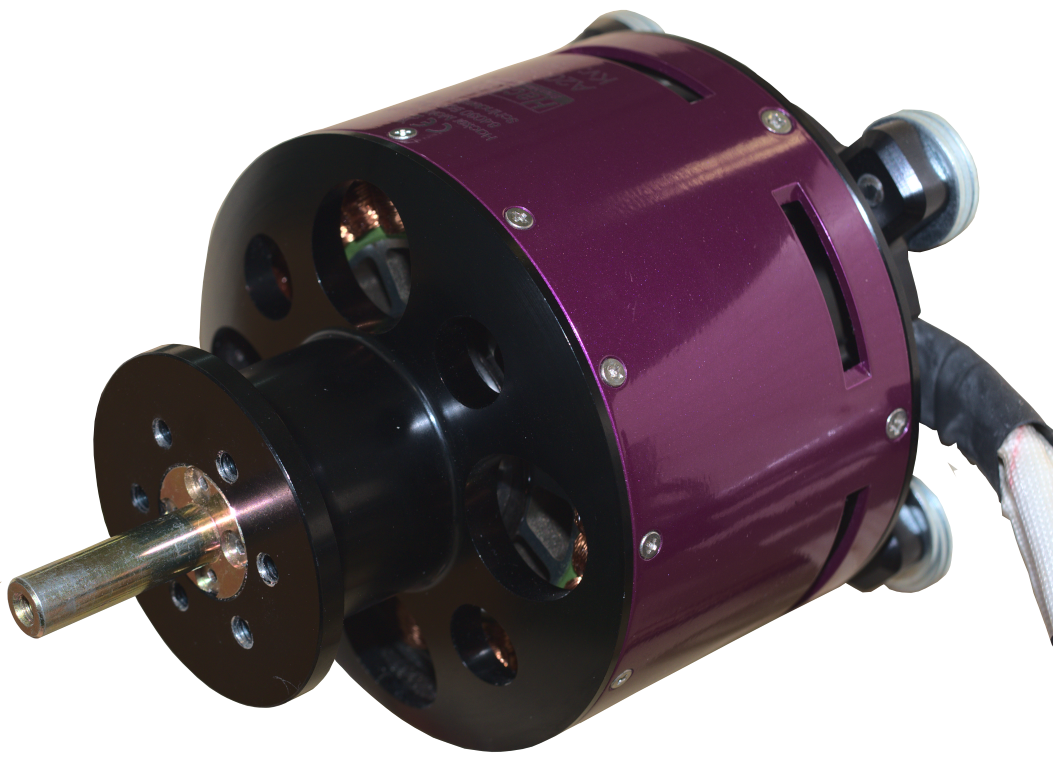
\includegraphics[width=0.5\textwidth]{Fotos/Motor.png}
    \caption{Hacker A200 Elektromotor}
\end{figure}
\todo[]{Text und Bilder zu Motoren einfügen}
\newpage
\section{Motorregler}
Die Ansteuerung der Motoren übernimmt der dafür empfohlene \textbf{MasterSpin 220 Pro OPTO}.
\begin{figure}[h]
    \centering
    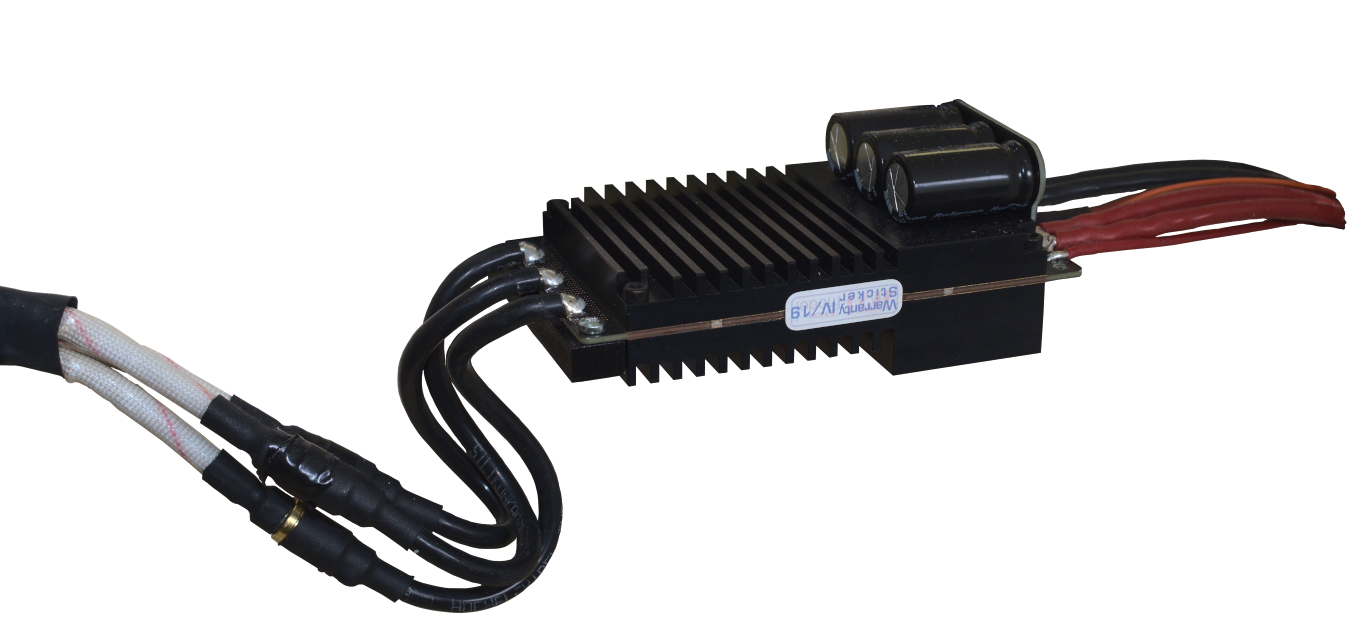
\includegraphics[width=0.9\textwidth]{Fotos/MasterSpin_ohne_Halter.png}
    \caption{MasterSPIN 220 Pro OPTO}
\end{figure}
\subsection*{Parametrierung durch JetiBox}
Um den Regler auf unsere Bedürfnisse parametrieren zu können, wurde eine sogenannte "JetiBox" verwendet.
\begin{figure}[h]
    \centering
    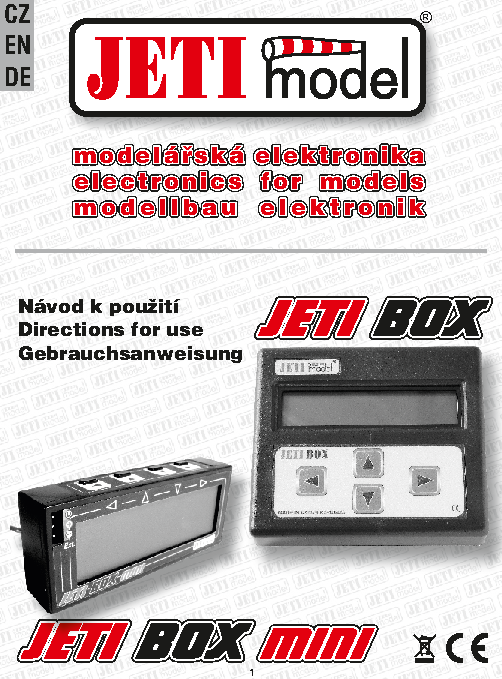
\includegraphics[width=0.5\textwidth]{Fotos/JetiBox.png}
    \caption{Jetibox}
\end{figure}
\newpage
Um in das Konfigurationsmenü des Reglers zu gelangen, muss die JetiBox am kürzeren der beiden 3-poligen Kabeln des MasterSpin 220 PRO OPTO angeschlossenen werden (Jenes mit dem roten Stecker), 
während man das PWM-Kabel (länger \& schwarzer Stecker) abgeschlossen hat.\\

Konkret wurden folgende Einstellungen getroffen:\\
\begin{table}[h]
\centering
\begin{threeparttable}
    
    \begin{tabular}{|l|l|}
    \hline
     Menüpunkt & getroffene Einstellung \\\hline
     Temp. Protection & $90\,^\circ\,\textrm{C}$\\
     Brake & Hard 70/100/0,5s\\
     Operation Mode & Fast Response\\
     Autorotation & OFF\\
     Timing & $22^\circ$\\
     Frequency & 8 kHz\\
     Acceleration & 0-100\% 5,0 s\\
     Accumulator Type & Li-Ion/Pol/Fe\\
     Number of Cells & Li-XX 14\\
     Li-XX Cut OFF & V Per Cell 3.2\\
     Off Voltage Set & 44,75 V\\
     Cut OFF & Slow Down\\
     Initial Point & AUTO\\
     END Point & 2.05 ms / 2.15 ms \tnote{1}\\
     AutoInc.END Poin & OFF(FIX)\\
     Throttle Curve & Linear\\
     Rotation & Left \tnote{2}\\
     Start-up Power & Auto\\
     Setting th. R/C & OFF\\\hline
    \end{tabular}
    \begin{tablenotes}\footnotesize 
        \item[1] 2.15 ms zur Begrenzung der Motorleistung auf \\$\approx 90\%$
        \item[2] Abhängig von der Verkabelung des Motors 
        \end{tablenotes}
    \end{threeparttable}
    \caption{Durch JetiBox am Regler konfigurierte Parameter}
\end{table}

\newpage